\documentclass[
	11pt,
	aspectratio=169,
]{beamer}

% Setting the colors
\hypersetup{
	colorlinks,
	citecolor=cyan,
	linkcolor=.,
	urlcolor=cyan
}
\usepackage[utf8]{inputenc}
\usepackage[T1]{fontenc}

% Remove these 2 lines
\usepackage[english]{babel}
\usepackage{blindtext}

% Defining a color
\usepackage{xcolor}
\definecolor{uwo-purple}{HTML}{4F2683}
\definecolor{uwo-gray}{HTML}{807F83}

% Refs
\usepackage[backend=bibtex,style=alphabetic]{biblatex}
\addbibresource{refs.bib}

% Phonetic characters
\usepackage{tipa}
\usepackage{tipx}



\usetheme{CambridgeUS}

% Customizing the template
\setbeamercolor{frametitle}{fg=uwo-purple}
\setbeamercolor{title}{fg=uwo-purple}
\setbeamercolor{palette primary}{fg=black, bg=uwo-purple!30!white}
\setbeamercolor{palette secondary}{fg=black, bg=uwo-purple!20!white}
\setbeamercolor{palette tertiary}{bg=uwo-purple}


\begin{document}
	\author{Amir HaghighatiMaleki}
	\title{Design/Cybernetics: Two Sides of One Coin}
	\subtitle{Reading Course Presentation}
	\logo{
\includegraphics[width=0.7cm]{resources/uwo-purple.png}}
	\institute{Insight Lab}
	\date{\today}
	\subject{Reading Course Presentation}
	%\setbeamercovered{transparent}
	%\setbeamertemplate{navigation symbols}{}
	\begin{frame}
		\maketitle
		\centering\tiny\hyperlink{http://insight.uwo.ca}{insight.uwo.ca}\\
		\centering\tiny\hyperlink{mailto:ahaghig3@uwo.ca}{ahaghig3@uwo.ca}
	\end{frame}

    \begin{frame}
    	\textit{\rm``The progress of knowledge is at the same time the progress of ignorance.''}\\
    	--- Edgar Morin \cite{morin_1992} \\
    	\vspace{0.4cm}
    	\textit{\rm``The very act of focusing prevents us from seeing.''}\\
    	--- ?? \\
    	\vspace{0.4cm}
    	\textit{\rm``We do not see what we do not see, and what we do not see seems nonexistent.''}\\
    	--- Humberto R. Maturana and Francisco J. Varela \cite{maturana_varela_1987}\\
    	\vspace{0.4cm}
    	\textit{\rm``The only way to overcome second-order deficiencies is with therapies of second order.''}\\
    	--- Heinz von Foerster \cite{vonFoerster_2003}\\
    	\vspace{0.4cm}
    	\begin{figure}
    		\centering
    		\href{https://anewage.github.io}{
    			
\includegraphics[width=2cm]{resources/anewage_github_io.png}
    		}
    	\end{figure}
    \end{frame}

    \section*{Prolouge}
        \begin{frame}
        	\frametitle{Prologue I}
        	\begin{columns}
        		\column{0.3\textwidth}
        			\begin{figure}
        				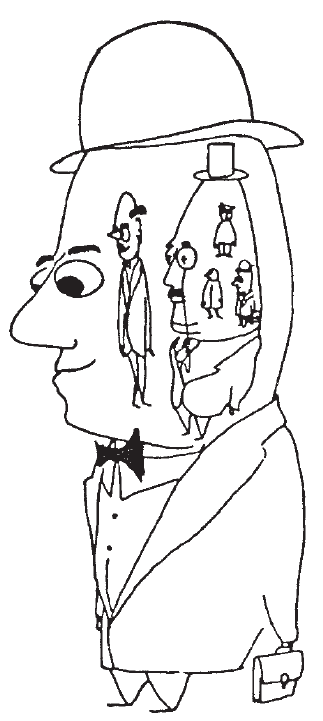
\includegraphics[height=0.7\textheight]{resources/man.png}
        			\end{figure}
        		\column{0.3\textwidth}
        			\begin{figure}
        				
\includegraphics[width=\textwidth]{resources/liar.jpg}
        			\end{figure}
        		\column{0.3\textwidth}
        			\begin{figure}
        				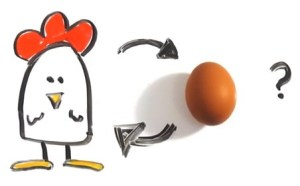
\includegraphics[width=\textwidth]{resources/chickenegg.jpg}
        			\end{figure}
        	\end{columns}
        \end{frame}

        \begin{frame}
        \frametitle{Prologue II}
        	{\textbf{Gödel's incompleteness} theorems can be summarized as: \\
        		It is impossible to construct a theoretical language that will not \textcolor{teal}{close on itself}, with the result that there are statements that are \textcolor{teal}{undecidable} in that language.} \\
        	\vspace{0.5cm}
        	{Simply put: There are things that you \textcolor{teal}{cannot explain within a paricular language}.}
        	
        \end{frame}

    \section*{Overview}
    	\begin{frame}
		\frametitle{Agenda}
    		\tableofcontents
    	\end{frame}

    \section{Introduction}
        \subsection{Initial Notes}
            \begin{frame}{Design}
                \framesubtitle{Basics}
                The word \textcolor{teal}{design} has its roots in drawing and designation. \\
        	    \textbf{As a noun} $\longrightarrow$ From Italian \textit{\rm designò}: ``to draw''\\
        	    \textbf{As a verb} $\longrightarrow$ From Latin \textit{\rm designare}: ``to designate, to outline, to appoint''\\
        	    \centering dē- (from, out) + signō (``to mark, to sign''). 
            \end{frame}
            \begin{frame}{Design}
                \framesubtitle{Wide Range of Approaches}
        		\begin{itemize}
        			\item<1->Design as a complex but essentially \textbf{mechanical} action (e.g., some approaches in Software Engineering, Herbert Simon):\\
        			    Assuming a set of specified criteria: design is generating a set of  alternatives and assessing them against the criteria
        			\item<2-> Horst Rittle (1973) $\longrightarrow$ design is essentially for \textcolor{teal}{``wicked problems''}:
        			\textbf{no definitive formulation}, \textbf{no stopping rule}, \textbf{no assessment criteria}
        			\item<3->Latest attempts: \textcolor{teal}{examine the heart of the design activity} instead of \textcolor{red}{prescription} and \textcolor{red}{proscription}: design and cognition (e.g., most interdisciplinary attempts)
        		\end{itemize}
            \end{frame}
            \begin{frame}{Cybernetics}
                \framesubtitle{Basics}
        			\textbf{Cybernetics} (\textbackslash \textipa{saI\texttt{}b@r"netIks}\textbackslash):
        			\begin{itemize}
        				\item<1-> From Greek `kybernetes': `\textcolor{teal}{steersman}'; `kybernan': `\textcolor{teal}{to steer or pilot a ship, direct as a pilot}'
        				\item<2-> Having a goal and taking action to achieve that goal
        				\item<3-> The art of steering \cite{pangaro_web}:
        			\end{itemize}
        			\centering\includegraphics<3>[width=7.2cm]{./resources/steering1.png}
        			\centering\includegraphics<4>[width=7.2cm]{./resources/steering2.png}
        			\centering\includegraphics<5>[width=7.2cm]{./resources/steering3.png}
        			\centering\includegraphics<6>[width=7.2cm]{./resources/steering4.png}
        			\centering\includegraphics<7>[width=7.2cm]{./resources/steering5.png}
        			\centering\includegraphics<8>[width=7.2cm]{./resources/steering6.png}
        			\centering\includegraphics<9>[width=7.2cm]{./resources/steering7.png}
        			\centering\includegraphics<10>[width=7.2cm]{./resources/steering8.png}
        			\centering\includegraphics<11>[width=7.2cm]{./resources/steering9.png}
        			\centering\includegraphics<12>[width=7.2cm]{./resources/steering10.png}
            \end{frame}
            \begin{frame}{Cybernetics}
                \framesubtitle{Approaches}
        		\begin{itemize}
        			\item<1-> \textcolor{teal}{Control}, \textcolor{teal}{feedback}, \textcolor{teal}{communication}, \textcolor{teal}{circular causality} $\longrightarrow$ from N. Wiener and the transdisciplinary endeavours at Macy Conferences (1946-1953):\\
        		    Many many forms -- applications in engineering, management, law, business, ...
        			\item<2-> When applied recursively to examine cybernetic ideas and institutions $\longrightarrow$ \textcolor{teal}{The cybernetics of} \textbf{\textcolor{teal}{observing}} (rather than \textcolor{orange}{observed}) systems: Second-Order Cybernetics\\
        			\textcolor{teal}{Constructive}, \textcolor{teal}{recursive}, and \textcolor{teal}{consistent} approach to cybernetics
        			\item<3-> Important figures and institutions: Kenneth Boulding, Margaret Mead, Heinz von Foerster, Gordon Pask, Humberto Maturana, Paul Pangaro, American Society for Cybernetics, International Society for the Systems Sciences, ...
        		\end{itemize}
            \end{frame}
            \begin{frame}{Cybernetics}
                \framesubtitle{Types of Systems \cite{pangaro_web}}
        		\begin{figure}
        		    \centering
        		    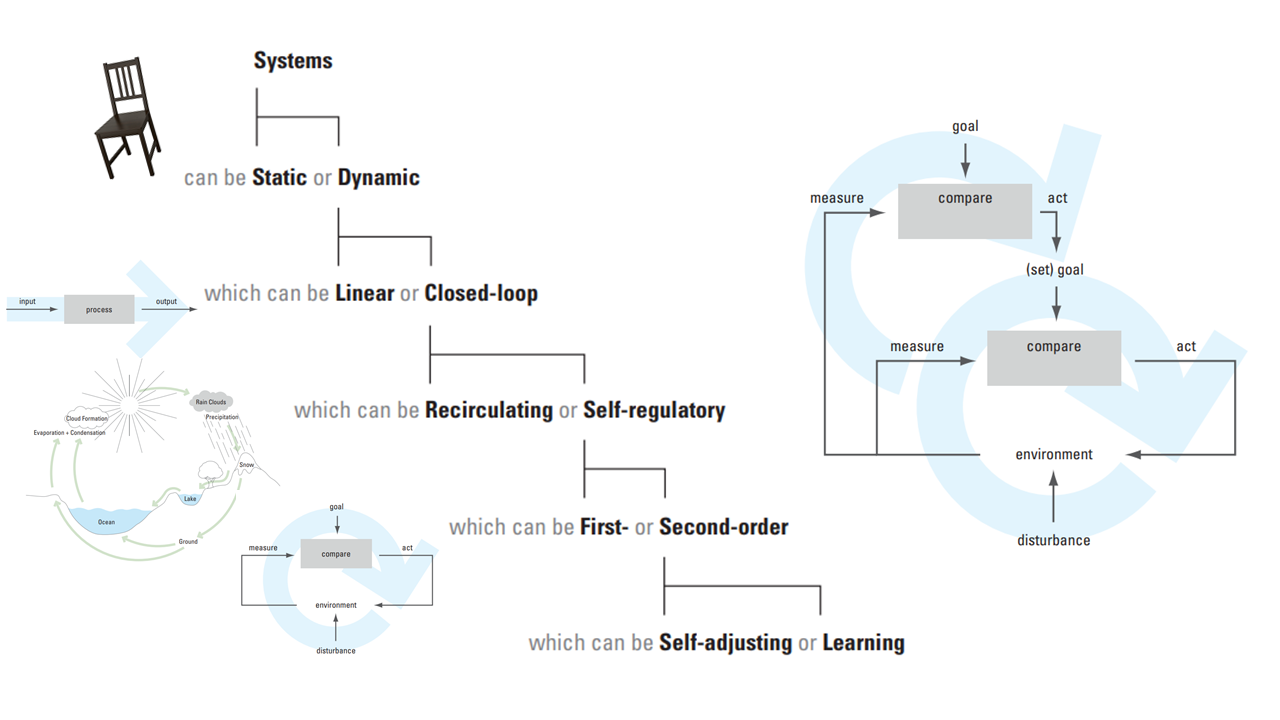
\includegraphics[height=0.75\textheight]{resources/systems.PNG}
        		\end{figure}
            \end{frame}
    \section{Considerations}
        \subsection{Design}
            \begin{frame}{Design}
                From this perspective, design is:
                \begin{itemize}
                    \item<1-> Not the outcome of a process.
                    \item<2-> Not a problem solving process.
                    \item<3-> Not a way of facing complexity.
                    \item<4-> An \textcolor{teal}{activity} that is carried out in the face of very complex and conflicting requirements.
                \end{itemize}
            \end{frame}
        \subsection{First-Order Cybernetics}
            \begin{frame}{Control}
                \begin{itemize}
                    \item<1-> Control \neq Restriction
                    \item<2-> Control = Guide towards better performance
                    \begin{itemize}
                        \item Goal or Intention
                        \item Means of communication of \textcolor{teal}{the intention} and \textcolor{teal}{the action of control} to an actor
                    \end{itemize}
                    \item<3-> What constitutes control in a system that \textcolor{teal}{enables} rather than \textcolor{red}{restricts}?
                \end{itemize}
            \end{frame}
            \begin{frame}{Law of Requisite Variety (First Law of Cybernetics)}
                \begin{itemize}
                    \item<1-> Variety = the number of all possible states for a system
                    \item<2-> Ross Ashby's law of \textcolor{teal}{Requisite Variety}: \\
                        In order to maintain its viability, the system that is in control must have at least as many states as the system to be controlled.
                    \item<3-> Not being restrictive $\longrightarrow$ The controller must have requisite variety.
                \end{itemize}
            \end{frame}
            \begin{frame}{Back to Control}
                \begin{columns}
                    \column{0.6\textwidth}
                        \begin{itemize}
                            \item<1-> In circular systems, which element controls and which is being controlled?
                            \item<2-> Control is \textcolor{red}{neither} in one element \textcolor{red}{nor} the other; it \textcolor{teal}{emerges} as a result of their \textcolor{teal}{interaction}.
                            \item<3-> Circularity is embodied in the role of the observer in cybernetic systems:\\
                            $\longrightarrow$ The observer cannot be inactive, or there would be no system.
                        \end{itemize}
                    \column{0.4\textwidth}
                    \begin{figure}
        		        \centering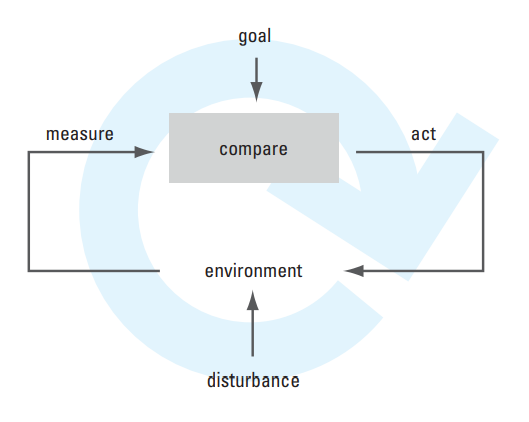
\includegraphics[height=0.6\textheight]{resources/thermostate.PNG}
        		    \end{figure}
                \end{columns}
            \end{frame}
        \subsection{Circularity and Second-Order Cybernetics}
            \begin{frame}{Subject/Metasubject}
                \begin{columns}
                    \column{0.5\textwidth}
                        \begin{itemize}
                            \item<1-> Mathematics:\\
                                A Distinct field worthy of consideration in its own right and by its own criteria.\\
                                Its \textcolor{teal}{abstraction} $\longrightarrow$ when applied to other subjects, \textcolor{teal}{casts light} upon them and \textcolor{teal}{enhances} our understanding.
                            \item<2-> Cybernetics $\sim$ Mathematics\\
                                Second-Order Cybernetics $\longrightarrow$ It is both its own subject and its own metasubject.
                            \item<3-> Design $\sim$ Cybernetics\\
                                Studied in the light of its own criteria:\\
                                (recursive) design of design
                        \end{itemize}
                    \column{0.5\textwidth}
                        \begin{itemize}
                            \item<4-> Cybernetics: \textcolor{teal}{structure} and \textcolor{teal}{form} to construct \textcolor{orange}{individual} meaning and understanding\\
                                Leaves \textcolor{teal}{meaning} and \textcolor{teal}{emotion} to the observer (\textcolor{red}{private})\\
                                $\longrightarrow$ Supports structures that support our \textcolor{teal}{autonomy} and \textcolor{teal}{freedom}\\
                                $\longrightarrow$ (recursive) \textcolor{teal}{Support of support}
                        \end{itemize}
                \end{columns}
            \end{frame}
            \subsubsection{Subjective/Objective}
                \begin{frame}{Subjective/Objective}
                    \framesubtitle{Observer Incorporated? \cite{vonFoerster_2003}}
                    \begin{columns}
                        \column{0.7\textwidth}
                            \begin{itemize}
                                \item<1-> Feedback $\longrightarrow$ an active actor (observer)
                                \item<2-> A description (observation) $\implies$ a describer (observer)
                                    \begin{enumerate}
                                        \item Observations are \textcolor{red}{not absolute} but \textcolor{teal}{relative} to the observer's point of view (Einstein)
                                        \item Observations \textcolor{teal}{affect} the observer to obliterate her hope of prediction (Heisenberg)
                                    \end{enumerate}
                                \item<3-> A description (of the world) $\implies$ a universal reality
                                \item<4-> A description (theory) of a describer has to account the \textcolor{teal}{describer} herself and her \textcolor{teal}{expression of the description}.
                            \end{itemize}
                        \column{0.3\textwidth}
                            ``I am a liar'' -- true or false? \\
                            \begin{figure}
                				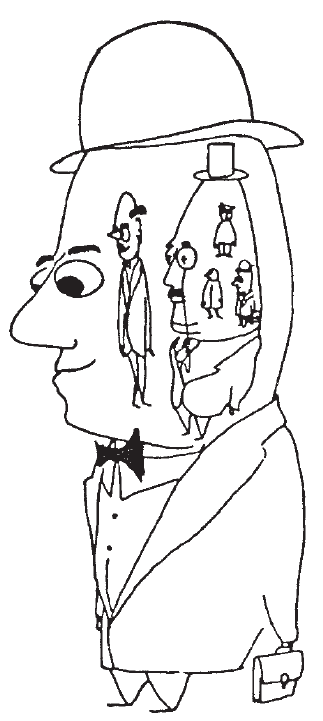
\includegraphics[height=0.5\textheight]{resources/man.png}
                			\end{figure}
                			``The reality is only my imagination'' (?)
                    \end{columns}
                \end{frame}
            \subsubsection{Recursion/Repetition}
                \begin{frame}
                    \frametitle{Recursion/Repetition}
                    \framesubtitle{Heinz von Foerster's Eigen Forms (structures, functions, objects, behaviours, and values)}
                    Tokens for stable behaviour: tokens for Eigen functions (Recursive Function Theory)\\
                    Examples:
                    \begin{itemize}
                        \item<1-> $f(x)= {{x}\over{2}} +1$\\
                            \fontsize{8}{9.2}\selectfont
                            \begin{columns}
                                \column{0.1\textwidth}
                                \column{0.4\textwidth}
                                    $\longrightarrow x_0=4$\\
                                    $\longrightarrow x_1=f(x_0) = {{4}\over{2}} + 1 = 3$ \\
                                    $\longrightarrow x_2=f(x_1) = {{3}\over{2}} + 1 = 2.5$ \\
                                    $\longrightarrow x_3=f(x_2) = {{2.5}\over{2}} + 1 = 2.25$\\
                                    $\longrightarrow x_4=f(x_3) = {{2.25}\over{2}} + 1 = 2.125$\\
                                    $\longrightarrow x_5=f(x_4) = {{2.125}\over{2}} + 1 = 2.063$\\
                                    $\longrightarrow x_{11}=f(x_{10}) = {{x_{10}}\over{2}} + 1 = 2.001$\\
                                    $\longrightarrow x_\infty=f(x_\infty) = {{x_\infty}\over{2}} + 1 = \textcolor{red}{2.000}$\\
                                \column{0.5\textwidth}
                                    $\longrightarrow x_0=1$\\
                                    $\longrightarrow x_1=f(x_0) = {{1}\over{2}} + 1 = 1.5$ \\
                                    $\longrightarrow x_2=f(x_1) = {{1.5}\over{2}} + 1 = 1.75$ \\
                                    $\longrightarrow x_3=f(x_2) = {{1.75}\over{2}} + 1 = 1.875$\\
                                    $\longrightarrow x_8=f(x_7) = {{x_7}\over{2}} + 1 = 1.996$\\
                                    $\longrightarrow x_{10}=f(x_9) = {{x_9}\over{2}} + 1 = 1.999$\\
                                    $\longrightarrow x_\infty=f(x_\infty) = {{x_\infty}\over{2}} + 1 = \textcolor{red}{2.000}$\\ 
                            \end{columns}
                        \item<2-> $2$ is the \textcolor{teal}{Eigen value} of $f$
                    \end{itemize}
                \end{frame}
                \begin{frame}
                    \frametitle{Recursion/Repetition}
                    \framesubtitle{Heinz von Foerster's Eigen Forms (structures, functions, objects, behaviours, and values)}
                    Tokens for stable behaviour: tokens for Eigen functions (Recursive Function Theory)\\
                    Examples:
                    \begin{itemize}
                        \item<1-> $f(g)= {{d}\over{dx}}g$\\
                            $exp=e^x \implies f(exp) = {{d}\over{dx}}exp = exp$\\
                            $\longrightarrow f(f(f(...f(f(exp))...))) = exp$\\
                        \item<2-> $exp = e^x$ is the \textcolor{teal}{Eigen function} for operator $f$
                    \end{itemize}
                \end{frame}
                \begin{frame}
                    \frametitle{Recursion/Repetition}
                    \framesubtitle{Heinz von Foerster's Eigen Forms (structures, functions, objects, behaviours, and values)}
                    Tokens for stable behaviour: tokens for Eigen functions (Recursive Function Theory)\\
                    Examples:
                    \begin{itemize}
                        \item<1-> ``This sentence has ... letters'' $\implies$ \textcolor{red}{THIRTY-ONE} or \textcolor{red}{THIRTY-THREE}\\
                        ``This sentence \textcolor{blue}{`This sentence has THIRTY-ONE letters'} has ... letters'' $\implies$ \textcolor{red}{THIRTY-ONE}\\
                        ``This sentence \textcolor{purple}{`This sentence \textcolor{blue}{<This sentence has THIRTY-ONE letters>} has THIRTY-ONE letters'} has ... letters'' $\implies$ \textcolor{red}{THIRTY-ONE} \\
                        \vspace{0.7cm}
                        \item<2-> ``This sentence consists of ... letters'' $\implies$ THIRTY-NINE \\
                        ``This sentence is composed of ... letters'' $\implies$ $\nexists$
                    \end{itemize}
                \end{frame}
                \begin{frame}{Recursion/Repetition}
                    \framesubtitle{Learning, Autopoiesis, Eigen Forms, and Ranulph Glanville's Object Theory}
                    \begin{figure}
                        \centering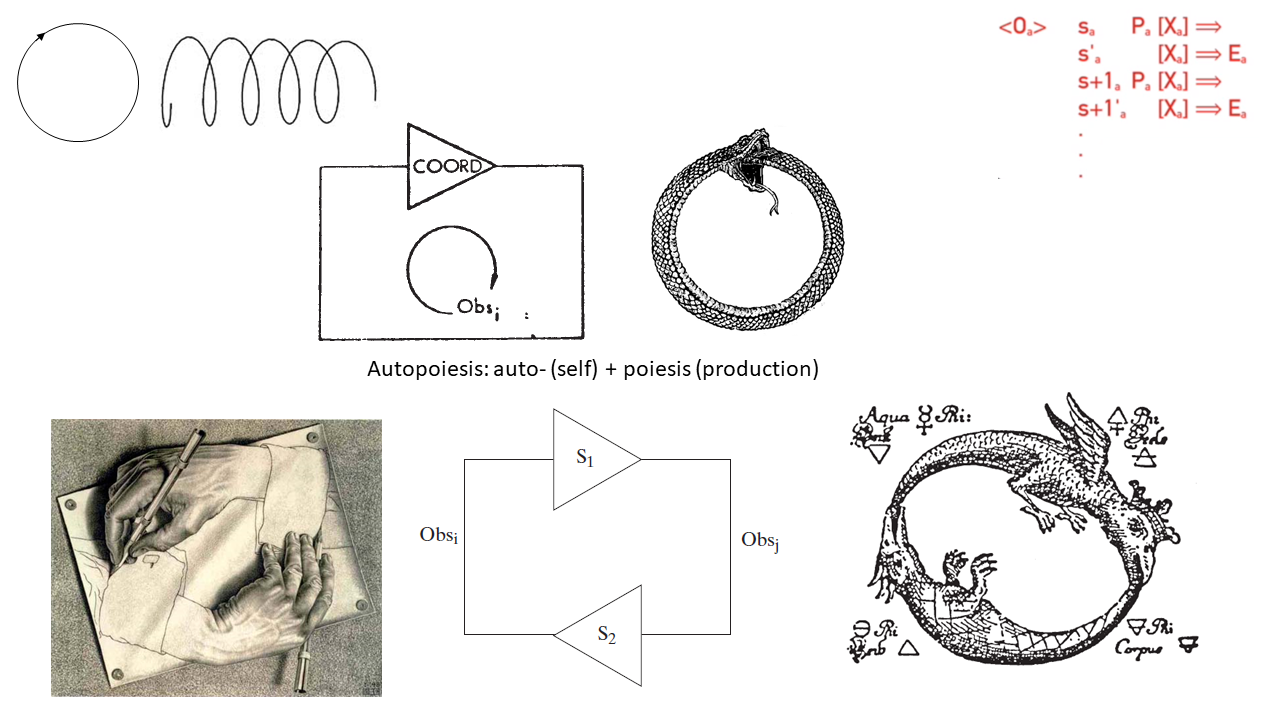
\includegraphics[width=0.7\textwidth]{resources/recursion.png}
                    \end{figure}
                \end{frame}
            \subsubsection{Conversation}
                \begin{frame}{Conversation Model \cite{pangaro_web}}
                    \framesubtitle{Based on Gordon Pask's Conversation Theory (1976)}
                    \centering\includegraphics<1>[page=23, width=0.75\textwidth]{resources/Pangaro-HCII_Seminar-April_2019-distro.pdf}
                    \centering\includegraphics<2>[page=24, width=0.75\textwidth]{resources/Pangaro-HCII_Seminar-April_2019-distro.pdf}
                    \centering\includegraphics<3>[page=25, width=0.75\textwidth]{resources/Pangaro-HCII_Seminar-April_2019-distro.pdf}
                    \centering\includegraphics<4>[page=26, width=0.75\textwidth]{resources/Pangaro-HCII_Seminar-April_2019-distro.pdf}
                    \centering\includegraphics<5>[page=27, width=0.75\textwidth]{resources/Pangaro-HCII_Seminar-April_2019-distro.pdf}
                    \centering\includegraphics<6>[page=28, width=0.75\textwidth]{resources/Pangaro-HCII_Seminar-April_2019-distro.pdf}
                    \centering\includegraphics<7>[page=29, width=0.75\textwidth]{resources/Pangaro-HCII_Seminar-April_2019-distro.pdf}
                    \centering\includegraphics<8>[page=30, width=0.75\textwidth]{resources/Pangaro-HCII_Seminar-April_2019-distro.pdf}
                    \centering\includegraphics<9>[page=31, width=0.75\textwidth]{resources/Pangaro-HCII_Seminar-April_2019-distro.pdf}
                    \centering\includegraphics<10>[page=32, width=0.75\textwidth]{resources/Pangaro-HCII_Seminar-April_2019-distro.pdf}
                    \centering\includegraphics<11>[page=33, width=0.75\textwidth]{resources/Pangaro-HCII_Seminar-April_2019-distro.pdf}
                    \centering\includegraphics<12>[page=34, width=0.75\textwidth]{resources/Pangaro-HCII_Seminar-April_2019-distro.pdf}
                \end{frame}
                \begin{frame}{The Theory}
                    \framesubtitle{Gordon Pask's Conversation Theory (1976)}
                    \centering\includegraphics<1>[page=99, width=0.75\textwidth]{resources/Pangaro-HCII_Seminar-April_2019-distro.pdf}
                \end{frame}
                \begin{frame}{Mental Models \cite{dubberly2009}}
                    \centering 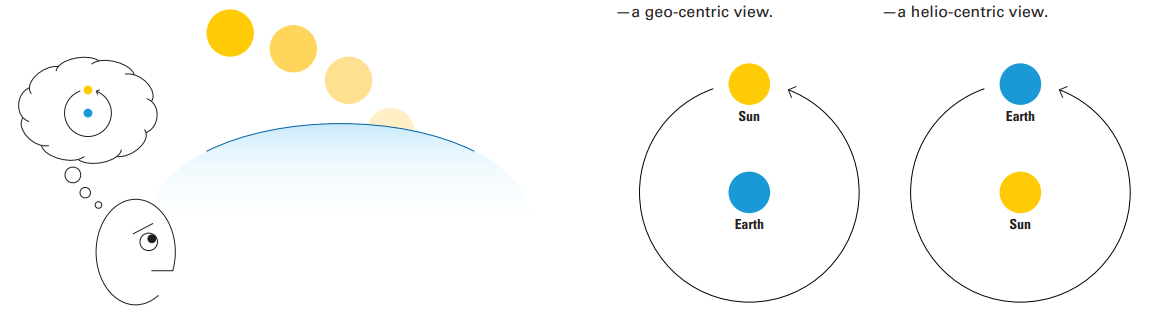
\includegraphics[width=\textwidth]{resources/models1.PNG}
                \end{frame}
                \begin{frame}{Mental Models \cite{dubberly2009}}
                    \framesubtitle{Learning as Forming and Reforming Models}
                    \centering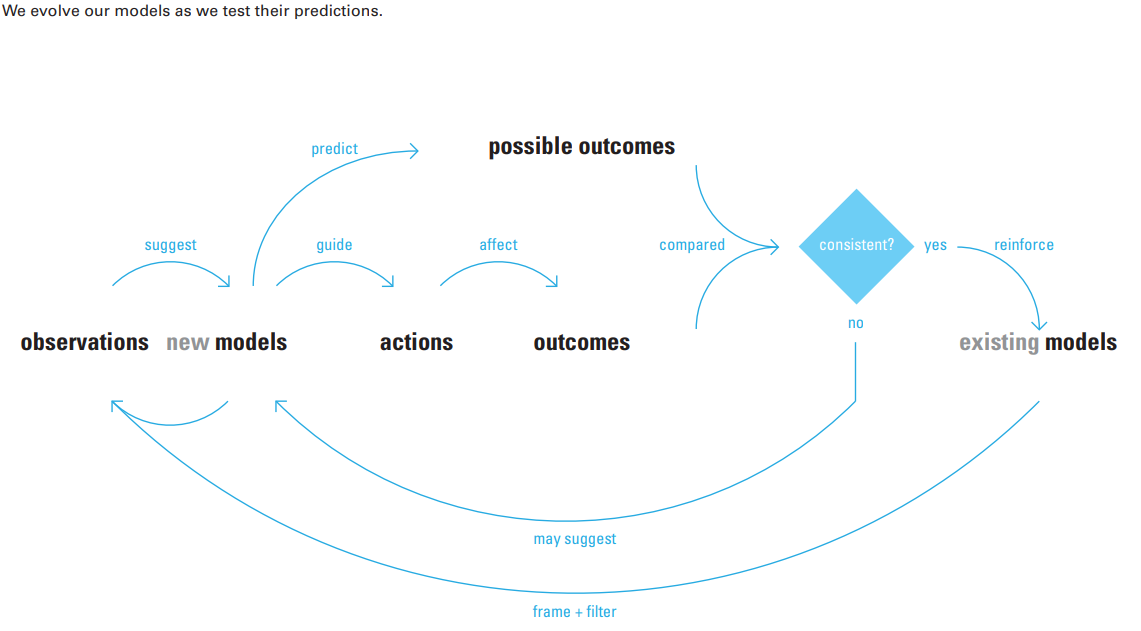
\includegraphics[width=0.75\textwidth]{resources/learning.PNG}
                \end{frame}
                \begin{frame}{Mental Models \cite{dubberly2009}}
                    \framesubtitle{TV dramas shape culture or culture inspire TV dramas?}
                    \centering\includegraphics<1->[width=0.75\textwidth]{resources/models4.PNG} \\
                    \centering\includegraphics<2->[width=0.25\textwidth]{resources/chickenegg.jpg}
                \end{frame}
                \begin{frame}{Mental Models \cite{dubberly2009}}
                    \framesubtitle{Agreement}
                    \centering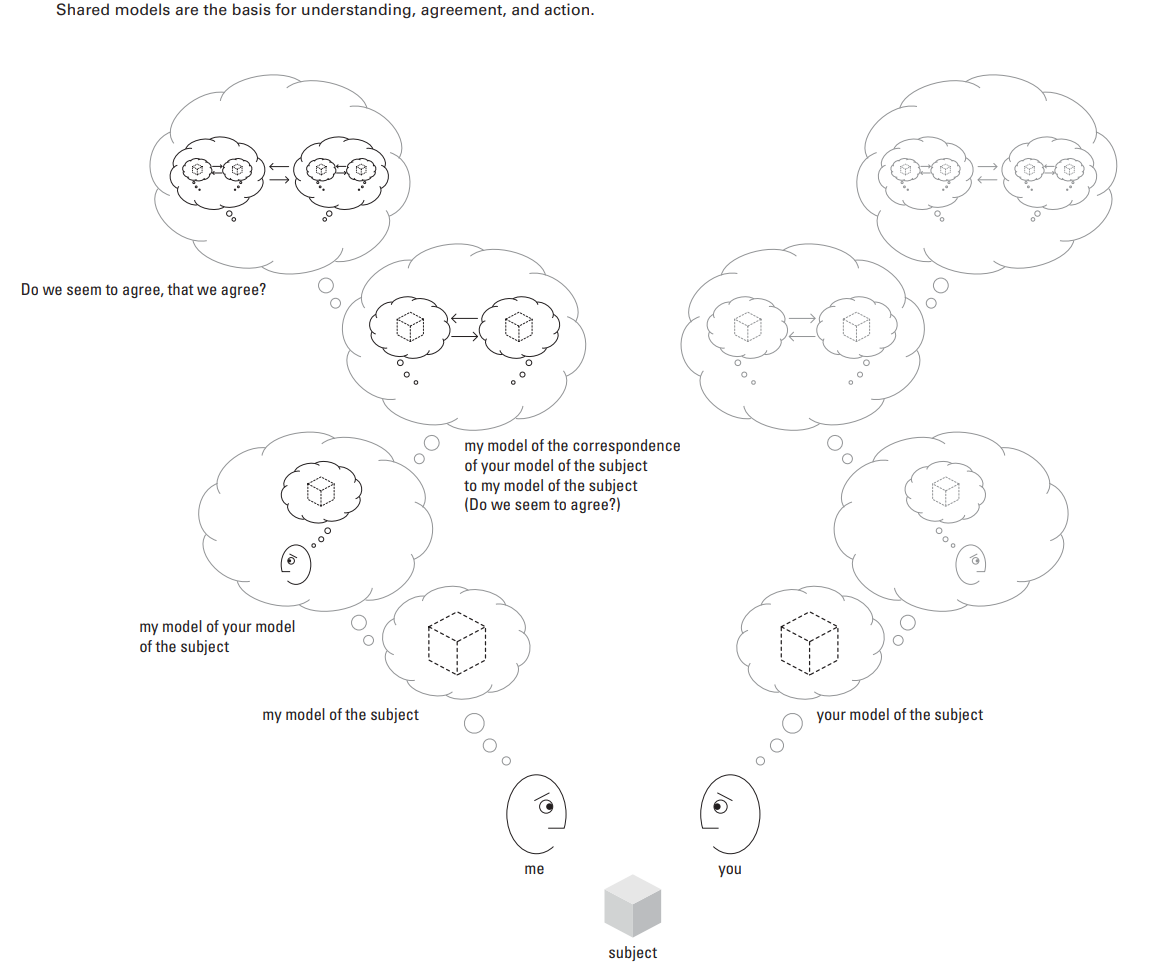
\includegraphics[width=0.5\textwidth]{resources/models5.PNG}
                \end{frame}
                \begin{frame}{Why Conversation? \cite{pangaro_web}}
                    \centering\includegraphics<1>[page=35, width=0.75\textwidth]{resources/Pangaro-HCII_Seminar-April_2019-distro.pdf}
                    \centering\includegraphics<2>[page=36, width=0.75\textwidth]{resources/Pangaro-HCII_Seminar-April_2019-distro.pdf}
                    \centering\includegraphics<3>[page=37, width=0.75\textwidth]{resources/Pangaro-HCII_Seminar-April_2019-distro.pdf}
                \end{frame}
    \section{The Harmony}
        \


\section{References}
	\begin{frame}[allowframebreaks]
		\frametitle{References}
		\printbibliography
	\end{frame}

\section*{Appendix}
	\begin{frame}
		\setbeamercovered{transparent}
		\frametitle{Definition(s) of Cybernetics}
		\framesubtitle{Soooo... What is Cybernetics?}
		\begin{itemize}
			\item<1->Ship of the State: The Command of a naval vessel is a metaphor for the governance of a city/state.\\
			--- Plato (420s-340s B.C.)
			\item<2->``Cybernetique is the art of governing or the science of government.''\\
			--- André-Marie Ampère (1775-1836)
			\item<3->``Use the word ‘cybernetics’, Norbert, because nobody knows what it means. This will always put you at an advantage in arguments.''\\
			Widely quoted; attributed to Claude Shannon in a letter to Norbert Wiener in the 1940s.
		\end{itemize}
		\setbeamercovered{invisible}
	\end{frame}
	\begin{frame}{What is NOT a Conversation?}
        \framesubtitle{Shannon's Model of Transmission}
        \begin{figure}
            \centering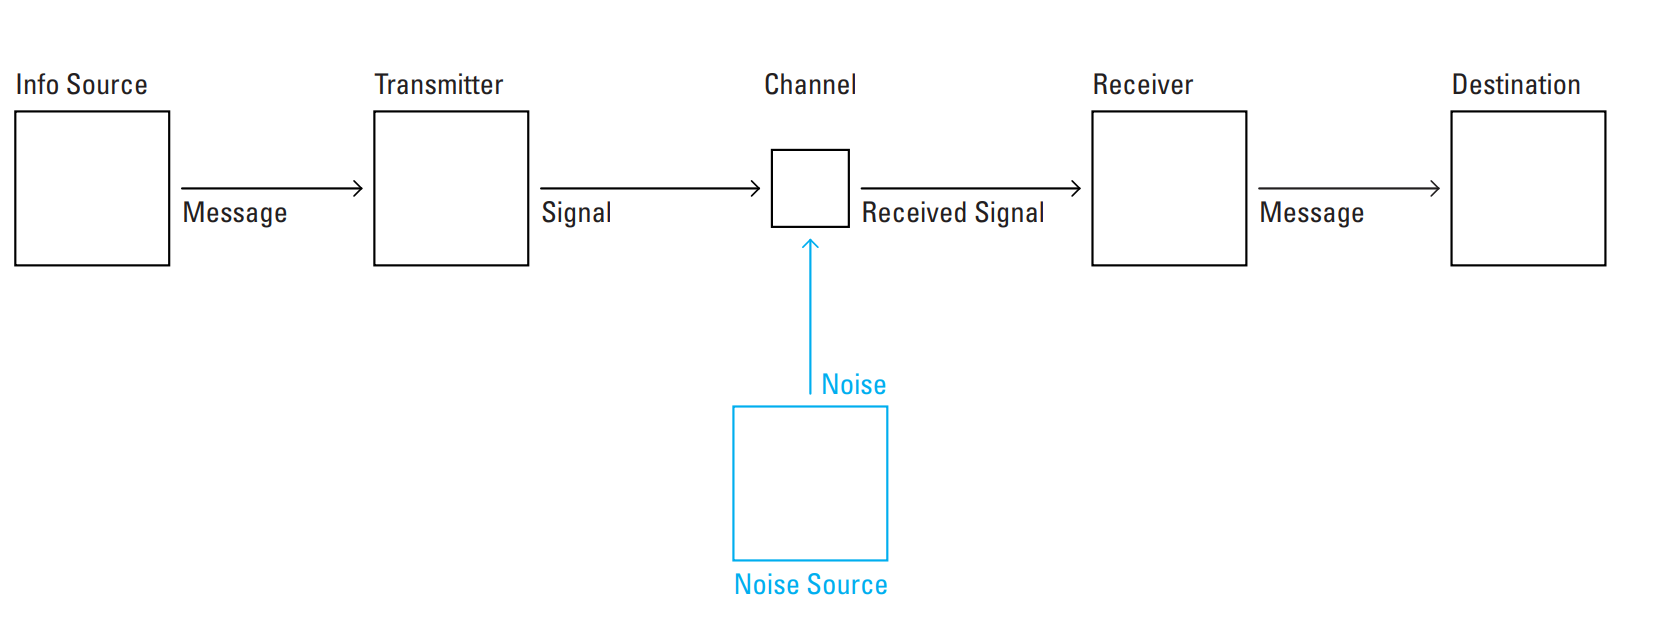
\includegraphics[width=0.8\textwidth]{resources/transmission.PNG}
        \end{figure}
        This model does not scaffold novelty, is pure mechanical, and does not support learning.
    \end{frame}
    \begin{frame}{Mental Models}
        \framesubtitle{Shaping and re-Shaping}
            \centering\includegraphics<1>[width=0.75\textwidth]{resources/models6.PNG}
            \centering\includegraphics<2>[height=0.77\textheight]{resources/models7.PNG}
    \end{frame}
    \begin{frame}{Interaction}
        \framesubtitle{Configurations \cite{pangaro_web}}
		\begin{figure}
		    \centering
		    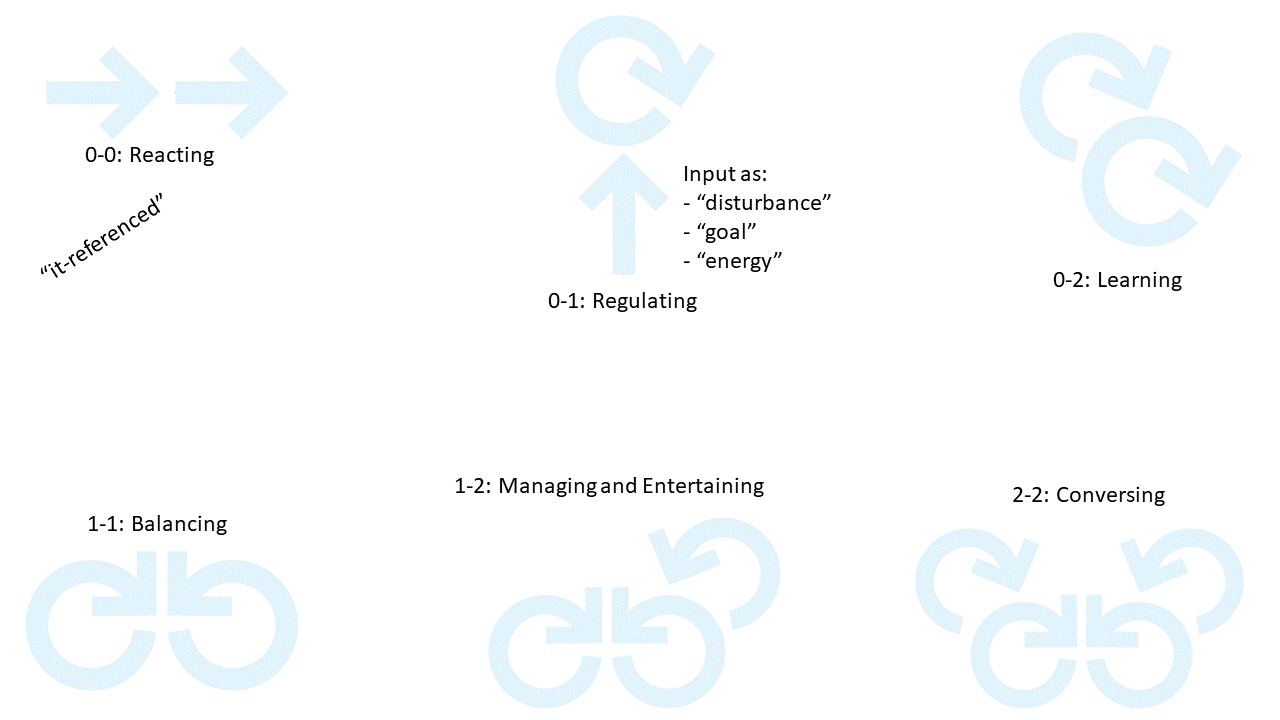
\includegraphics[height=0.75\textheight]{resources/interaction.PNG}
		\end{figure}
    \end{frame}
\end{document}